\documentclass[aspectratio=169,usenames,dvipsnames]{beamer}
\beamertemplatenavigationsymbolsempty
% \documentclass{beamer}

% UNCOMMENT FOR HANDOUTS
% \usepackage{pgfpages}
% \pgfpagesuselayout{2 on 1}[landscape,letterpaper,border shrink=5mm]
% \setbeameroption{show notes}

\mode<presentation>
\usetheme{Boadilla}
\usecolortheme{spruce}
\usepackage{../../LizStyle,ulem}
\usepackage{color}
\usepackage[color,matrix,arrow]{xy}
% \input xy
% \xyoption{all}
\usepackage{tikz}
\usepackage{tikz-cd}
\tikzset{commutative diagrams/diagrams={ampersand replacement=\&}}

\AtBeginSection{\frame{\sectionpage}}


% ==========Command for putting comments and removing them=======
% Visible:
\newcommand{\InstructorNotes}[1]{\textit{\color{orange}#1}}
\newcommand{\InstructorList}[1]{
\begin{itemize}
	\color{orange}
	#1
\end{itemize}
}
% Removed:
%\renewcommand{\InstructorNotes}[1]{}
%\renewcommand{\InstructorList}[1]{}


\newcommand{\bvfill}{\vskip0pt plus 1filll}

\usepackage{multimedia}
\usepackage{graphbox}

% \usepackage{algpseudocode}


\newcommand{\Reeb}{\textbf{Reeb}}
\newcommand{\Rtopc}{\textbf{Rtopc}}
% \newcommand{\RR}{\mathcal{R}}

\newcommand{\Set}{\textbf{Set}}
\newcommand{\Vect}{\textbf{Vect}}
\newcommand{\Top}{\textbf{Top}}
\newcommand{\Int}{\textbf{Int}}


\graphicspath{ {Figures/} {../Figures/}{../../Figures/} }



\begin{document}
%\pdfoptionpdfminorversion 5
%\logo{\includegraphics[height=1.5cm]{dukeshield.pdf}}
\title[]{Ch 6.3: Dimension Reduction - PCA}
\subtitle{Lecture 19 - CMSE 381}
\date{Mon, March 9, 2026}



\institute[MSU-CMSE]{Michigan State University\\
			::\\
          Dept of Computational Mathematics, Science \& Engineering}


\begin{frame}
 \titlepage


\end{frame}
%--------------------------
\begin{frame}[c]{Announcements}

\begin{columns}
\column{.6\textwidth}
\centering

	\textbf{Last time:}
	\begin{itemize}
		\item Shrinkage: Ridge and Lasso
	\end{itemize}

	% \vspace{.2in}

	\textbf{This lecture:}
	\begin{itemize}
	\item PCA 
\end{itemize}
\textbf{Announcements:}
	\begin{itemize}
		\item Exam \#2 next week (Monday 3/16)! 
		\begin{itemize}
			\item Bring 8.5x11 sheet of paper 
			\item Handwritten both sides 
			\item Anything you want on it, but must be your work 
			\item Write your name and your group number
			\item You will turn it in
			\item Non-internet calculator
		\end{itemize} 
		\item Project: by Exam \# 2
		\begin{itemize}
			\item project partner, ideas about what method to use
		\end{itemize}
	\end{itemize}


\column{.5\textwidth}
\centering
	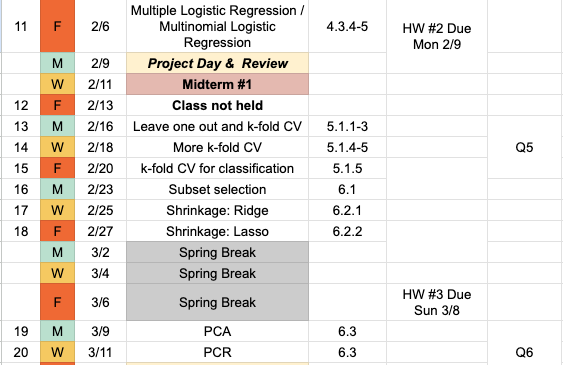
\includegraphics[width=0.8\textwidth]{Schedule-S26-Lecs11_to_20}
\end{columns}

\end{frame}
%--- Next Frame ---%

%=================
\section{Last time}
%=================

\begin{frame}[c]{Goal}

	\begin{columns}
	\column{.45\textwidth}
	\centering
	\begin{itemize}
		\item Fit model using all $p$ predictors
		\item Aim to constrain (regularize) coefficient estimates
		\item Shrink the coefficient estimates towards 0
	\end{itemize}
	\column{.45\textwidth}
	\centering
	
	\begin{equation*}
		Y = \beta_0 + \beta_1 X_1 + \beta_2 X_2 + \beta_3 X_3 + \beta_4 X_4
	\end{equation*}
	\InstructorList{
	\item Ridge regression
	\item Lasso
	}
	\end{columns}
	
	\end{frame}

%--- Next Frame ---%
\begin{frame}[t]{Shrinkage}
	Find $\beta$ to minimize:

	\bvfill 


\begin{columns}
\column{.3\textwidth}
\centering
\textbf{Least Squares:}\\
\footnotesize
\begin{equation*}
	RSS = \sum_{i=1}^n (y_i-\hat y_i)^2
	% \left(y_i - \beta_0 - \sum_{j=1}^p \beta_j x_{ij}\right)^2
\end{equation*}
% No constraints

\column{.3\textwidth}
\centering
\textbf{Ridge:}
\footnotesize
\begin{equation*}
	RSS +  \lambda \sum_{j=1}^p \beta_j^2
\end{equation*}

\column{.3\textwidth}
\centering

\textbf{The Lasso:}
\footnotesize
\begin{equation*}
	 RSS +\lambda \sum_{j=1}^p |\beta_j| 
\end{equation*}

\end{columns}

\bvfill

\begin{columns}
\column{.4\textwidth}
\centering
\includegraphics[width = \textwidth]{Fig6-4}
\column{.4\textwidth}
\centering

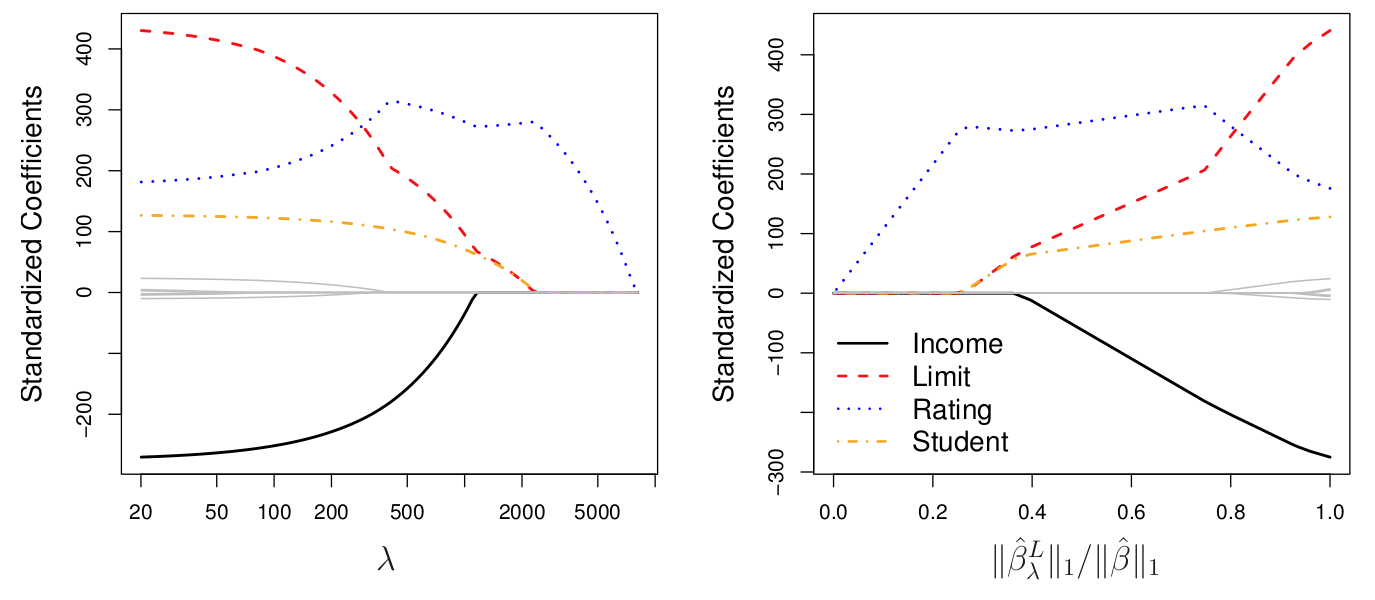
\includegraphics[width = \textwidth]{Fig6-6}
\end{columns}


\InstructorNotes{Also, find best choice of $\lambda$ or $s$ using CV}

\end{frame}
%--- Next Frame ---%

\begin{frame}[t]{What will you learn from this lecture?}
	\begin{itemize}
		\item How to create new variables as linear combinations of the original predictors?
		\item Why do we need Principal Component Analysis (PCA)? What is the main purpose of using it?
		\item What is a principal component (PC)?
		\item What does the first PC maximize? You should be able to explain this both geometrically in a plot and mathematically.
		\item Similarly, what do the subsequent PCs maximize?
		\item How do you compute the PCs in Python, given a dataset? 
		\item How do you project data points on each PC? You should also be able to plot the data points in the PC space. 
		\item How do you find out how much variance each PC explains?
	\end{itemize}

\end{frame}

%==========
\section{Dimension Reduction }
%==========


\begin{frame}[t]{Linear transformation of predictors }

\begin{columns}
\column{.45\textwidth}
\centering
Original Predictors:
\begin{equation*}
	X_1,\cdots,X_p
\end{equation*}
\column{.45\textwidth}
\centering
New Predictors:
\begin{equation*}
	Z_1,\cdots,Z_M
\end{equation*}
\begin{equation*}
	Z_m = \sum_{j=1}^p \phi_{jm}X_j
\end{equation*}

\end{columns}
\InstructorList{
\item The goal is for $M \ll p$
\item Need to figure out good $\phi$ to do this
}
\end{frame}
%--- Next Frame ---%

\begin{frame}[c]{An example or two}

\begin{columns}
	\column{.45\textwidth}
	\centering
\InstructorNotes{Two dimensions down to 1..... }
	\InstructorList{
	\item
		\begin{align*}
		Z_1 &= X_1 + 3 \cdot  X_2
	\end{align*}
	\item Matrix version:
	\begin{equation*}
		(Z_1) = 
		\begin{pmatrix}
			X_1 & X_2
		\end{pmatrix}
		\begin{pmatrix}
		1 \\ 3
		\end{pmatrix}
	\end{equation*}
	\item Example data:
	\begin{tabular}{cc|c}
		$X_1$ & $X_2$ & $Z_1$\\ \hline 
		0 & 1 & 3\\ 
		3 & 4 & 15 \\ 
		1 & 1 & 4 \\ 
		-1 & 0 & -1 
	\end{tabular}
	}


\column{.45\textwidth}
\centering
\InstructorNotes{Create an example with just three dimensions down to two}
\InstructorList{
\item $\phi = \begin{pmatrix}
1 & 0  \\
0 & 1/2 \\
0 & 1/2
\end{pmatrix}$
\begin{align*}
	Z_1 &= X_1 + 0 \cdot  X_2 + 0 \cdot X_3 \\
	Z_2 &= 0 \cdot X_1 + \tfrac{1}{2}X_2 + \tfrac{1}{2}X_3
\end{align*}
}


\end{columns}

\end{frame}
%--- Next Frame ---%
\begin{frame}[t]{Geometric interpretation}
\begin{columns}
\column{.45\textwidth}
\centering
\InstructorList{
	\item Get the $\phi$ to unit norm 
	\item Example: $Z_1 = \frac{1}{\sqrt{10}}X_1 + \frac{3}{\sqrt{10}}X_2 $
	\item Point out that the $Z$ value for the point is how far along the point projected down onto the line 
}
\begin{itemize}
	\item \href{https://www.geogebra.org/graphing/gucrrevt}{projection on a line}
\end{itemize}
\column{.45\textwidth}
\centering
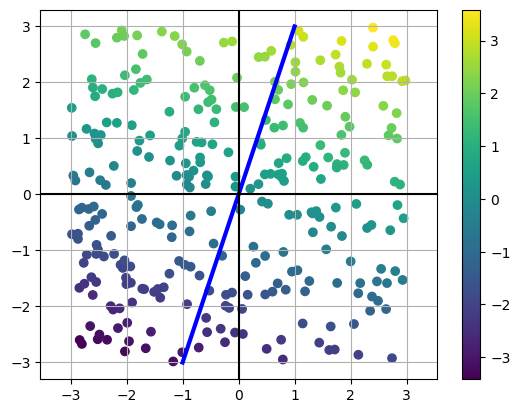
\includegraphics[align = c, width = \textwidth]{DimReduction_Projection.png}
% 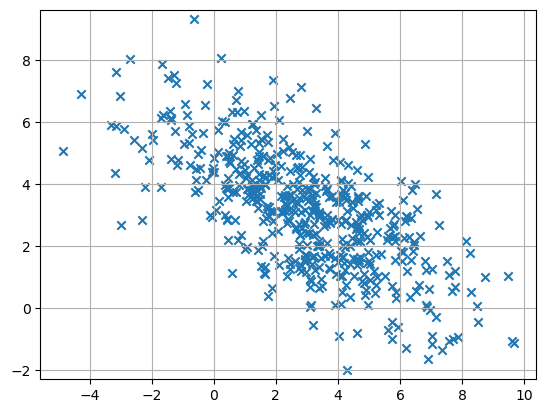
\includegraphics[align = c, width = \textwidth]{DimReduction_Projection_Example2.png}

\end{columns}
\end{frame}
%--- Next Frame ---%
% \begin{frame}[c]{Projection onto a line}

	% \begin{columns}
	% \column{.45\textwidth}
	% \centering
	% \url{https://www.desmos.com/calculator/cih7wy8oyg}
	% \column{.45\textwidth}
	% \centering
	
	% \end{columns}
	
	% \end{frame}

	%--- Next Frame ---%
	\begin{frame}[t]{Different projections}
	\begin{columns}
	\column{.3\textwidth}
	\centering
	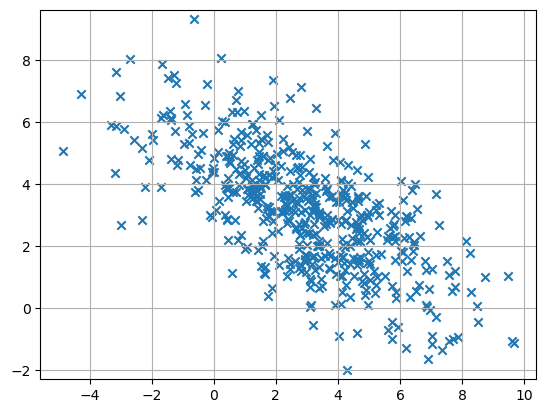
\includegraphics[align = c, width = \textwidth]
	{DimReduction_Projection_Example2.png} 
	% DimReduction_Projection_Example2_linecolor.png 
	% DimReduction_Projection_Example2_line.png
	\column{.55\textwidth}
	\centering
	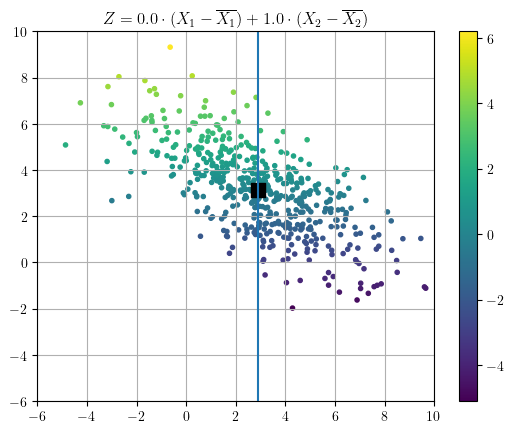
\includegraphics[align = c, width = .49\textwidth]{DimReduction_Projection_Example2_157.png} 
	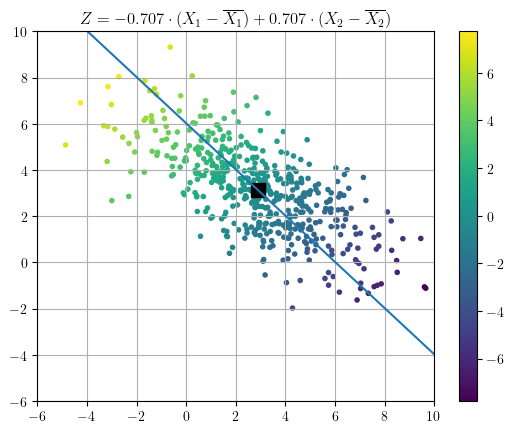
\includegraphics[align = c, width = .49\textwidth]{DimReduction_Projection_Example2_235.png} 
	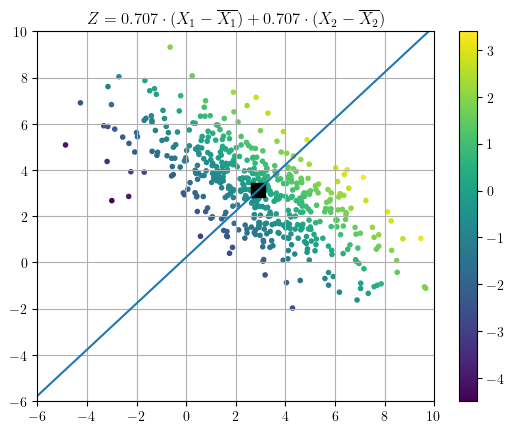
\includegraphics[align = c, width = .49\textwidth]{DimReduction_Projection_Example2_78.png} 
	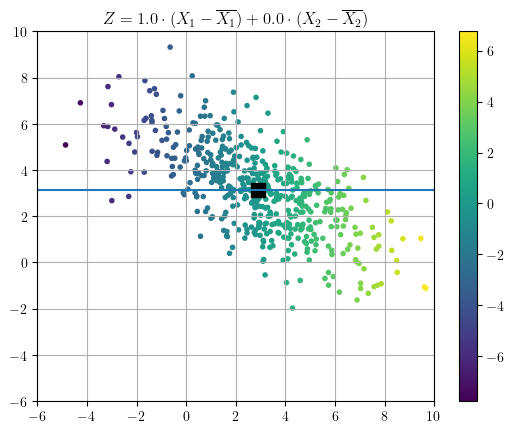
\includegraphics[align = c, width = .49\textwidth]{DimReduction_Projection_Example2_0.png} 
	\end{columns}
	\end{frame}
	%--- Next Frame ---%
	\begin{frame}[t]{Histograms of $Z$ values}
	\begin{columns}
	\column{.24\textwidth}
	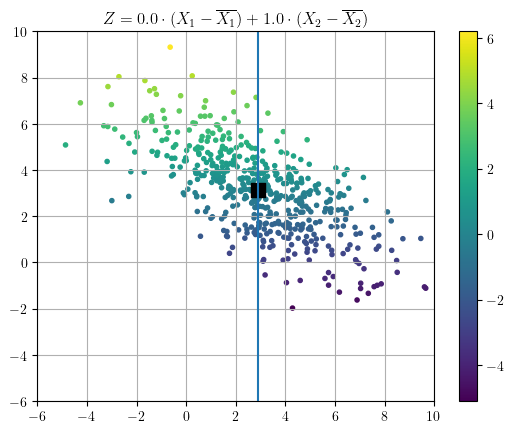
\includegraphics[align = c, width = \textwidth]{DimReduction_Projection_Example2_157.png} 
	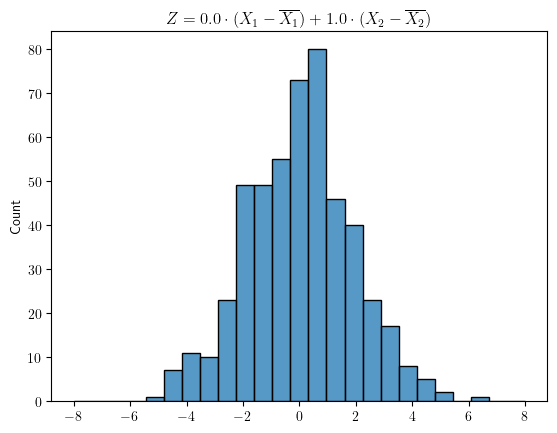
\includegraphics[align = c, width = \textwidth]{DimReduction_Projection_Example2_hist157.png} 
	
	\column{.24\textwidth}
	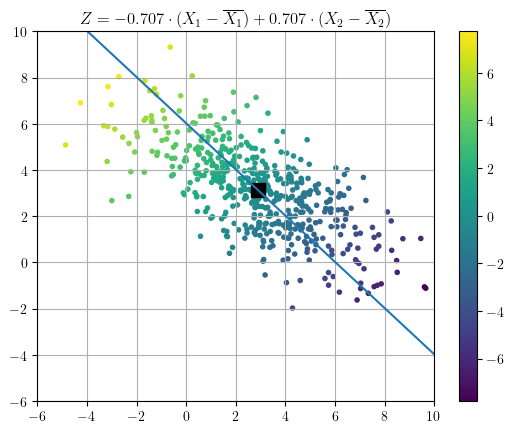
\includegraphics[align = c, width = \textwidth]{DimReduction_Projection_Example2_235.png} 
	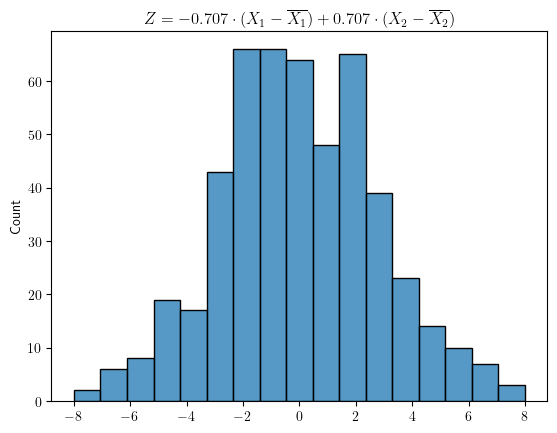
\includegraphics[align = c, width = \textwidth]{DimReduction_Projection_Example2_hist235.png} 

	\column{.24\textwidth}
	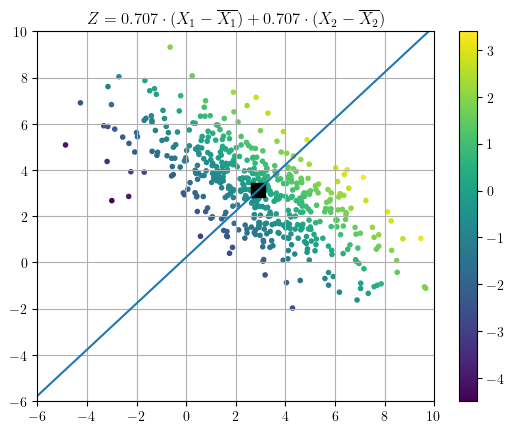
\includegraphics[align = c, width = \textwidth]{DimReduction_Projection_Example2_78.png} 
	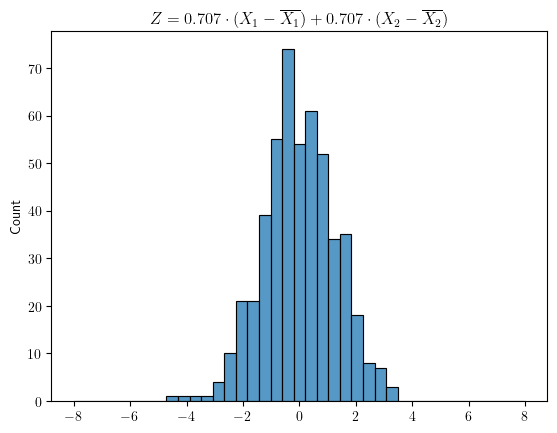
\includegraphics[align = c, width = \textwidth]{DimReduction_Projection_Example2_hist78.png} 

	\column{.24\textwidth}
	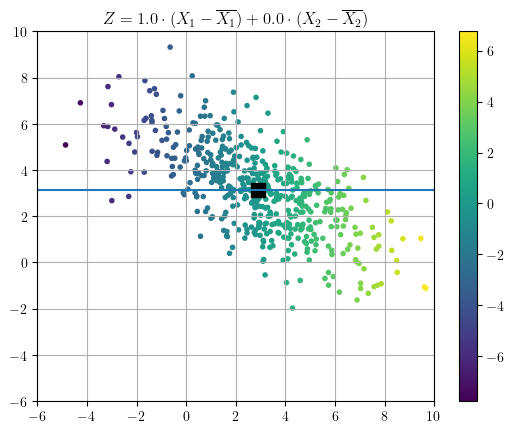
\includegraphics[align = c, width = \textwidth]{DimReduction_Projection_Example2_0.png} 
	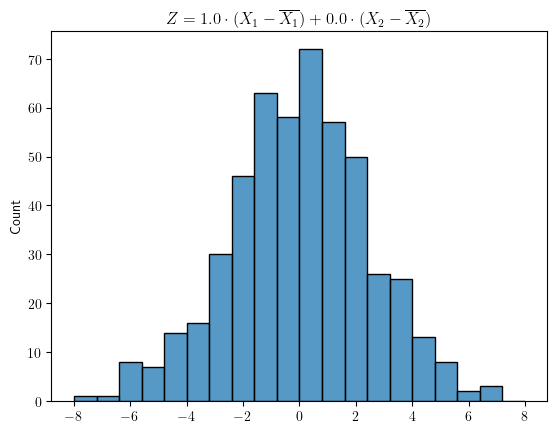
\includegraphics[align = c, width = \textwidth]{DimReduction_Projection_Example2_hist0.png} 
	\end{columns}
	\end{frame}
	%--- Next Frame ---%
\begin{frame}[c]{The goal}

\begin{columns}
\column{.45\textwidth}
\centering
\begin{itemize}
\item Find good $\phi$'s for some $M \ll p$
\item Fit regression model on $Z_i$'s using least squares
\begin{equation*}
	y_i = \theta_0 + \sum_{m=1}^M \theta_m z_{im} + \e_i
\end{equation*}
\end{itemize}
\InstructorList{
\item in this notation, $\theta$s replace $\beta$s

}
\column{.45\textwidth}
\centering
\InstructorList{
\item Dimension reduction comes from the fact that we're fitting models on a smaller number of variables
\item Next two subsection: ways to find $\phi$s: PCA and partial least squares
\item Today.... just PCA?
}
\end{columns}

\end{frame}
%--- Next Frame ---%

%==========
\section{PCA}
%==========

\begin{frame}[c]{An example dataset}

\begin{columns}
\column{.45\textwidth}
\centering
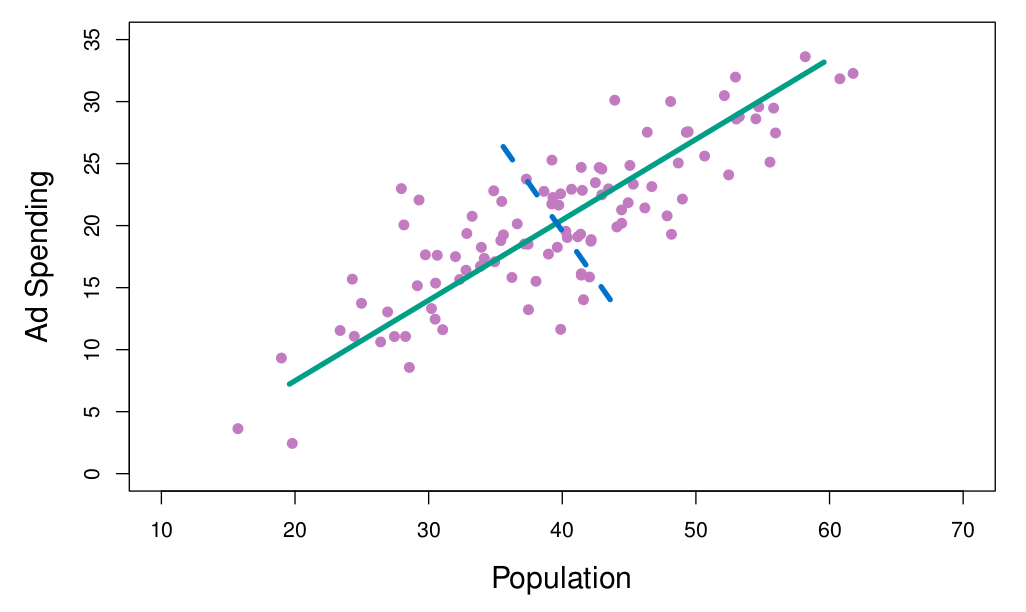
\includegraphics[width = \textwidth, align = c]{Fig6-14}
\column{.45\textwidth}
\centering
\InstructorList{
\item Population size in tens of thousands of people
\item Ad spending for a company in thousands of dollars
\item Note: These are both input variables
\item 100 data points
\item By eye: green line is the direction of most variability, called the principal component
\item Meaning if we project observations onto the line, then the projected observations would have the largest possible variance
\item
}
\end{columns}

\end{frame}
%--- Next Frame ---%





\begin{frame}[c]{Projection onto first PC}

	\centering
	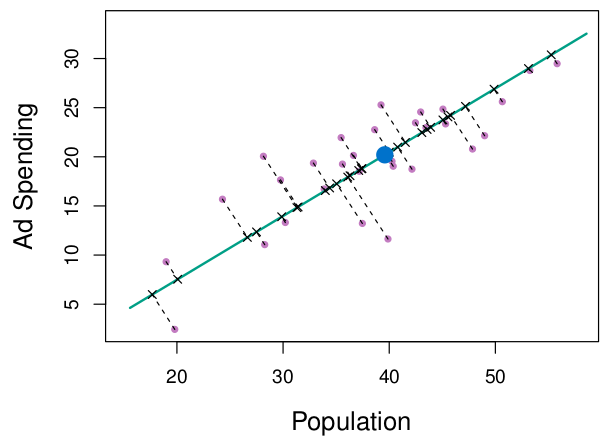
\includegraphics[width =.6 \textwidth, align = c]{Fig6-15a}

	\begin{equation*}
		Z_1 = 0.839 \cdot (\texttt{pop} - \overline{\texttt{pop}}) + 0.544 \cdot (\texttt{ad} - \overline{\texttt{ad}})
	\end{equation*}
	\InstructorNotes{$\phi_{11} = 0.839$ and $\phi_{21} = 0.544$ are the principal component loadings. Blue dot is $(\overline{pop},\overline{ad})$ }


\end{frame}
%--- Next Frame ---%


\begin{frame}[c]{What does it mean to have the highest variance}

\begin{columns}
\column{.45\textwidth}
\centering
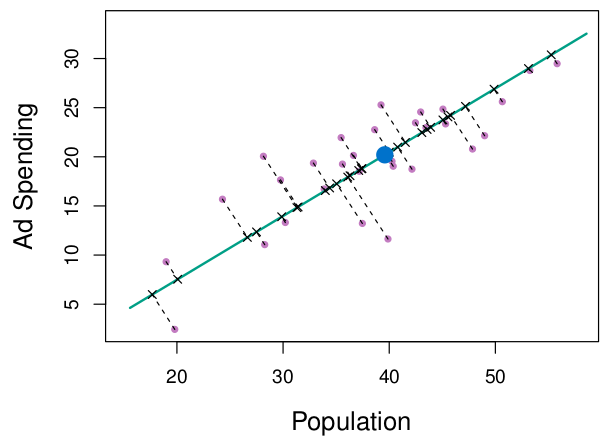
\includegraphics[width = \textwidth, align = c]{Fig6-15a}
\column{.45\textwidth}
\centering
\InstructorList{
\item Of every linear combo of pop and ad, this one has the highest variance
\item Maximizes $\Var(\phi_{1,1} (pop - \overline{pop}) + \phi_{2,1}(ad - \overline{ad}))$
\item Require $\phi_{11}^2 + \phi_{21}^2 = 1$, otherwise, just make $\phi$ super big to blow up variance
}
\end{columns}

\end{frame}
%--- Next Frame ---%
\begin{frame}[c]{Toy for learning PCA}

\begin{columns}
\column{.45\textwidth}
\centering
\url{https://www.desmos.com/calculator/gvmq07pg1k}
\column{.45\textwidth}
\centering
\InstructorNotes{
Don't forget to click step 2a to show points for PC2. 
}


\end{columns}

\end{frame}
%--- Next Frame ---%

\begin{frame}[c]{Principal component scores}

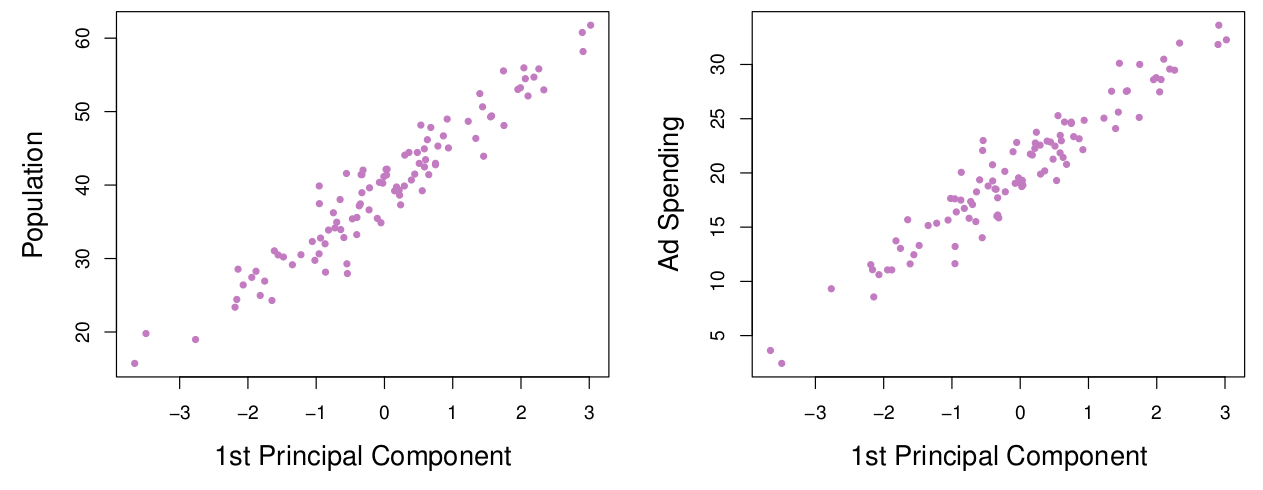
\includegraphics[width = \textwidth, align = c]{Fig6-16}
\begin{columns}
\column{.45\textwidth}
\centering
\begin{equation*}
	z_{i1} = 0.839 \cdot (\texttt{pop}_i - \overline{\texttt{pop}}) + 0.544 \cdot (\texttt{ad}_i - \overline{\texttt{ad}})
\end{equation*}
\column{.45\textwidth}
\centering

\end{columns}

\end{frame}
%--- Next Frame ---%


\begin{frame}[t]{Another view }

\centering
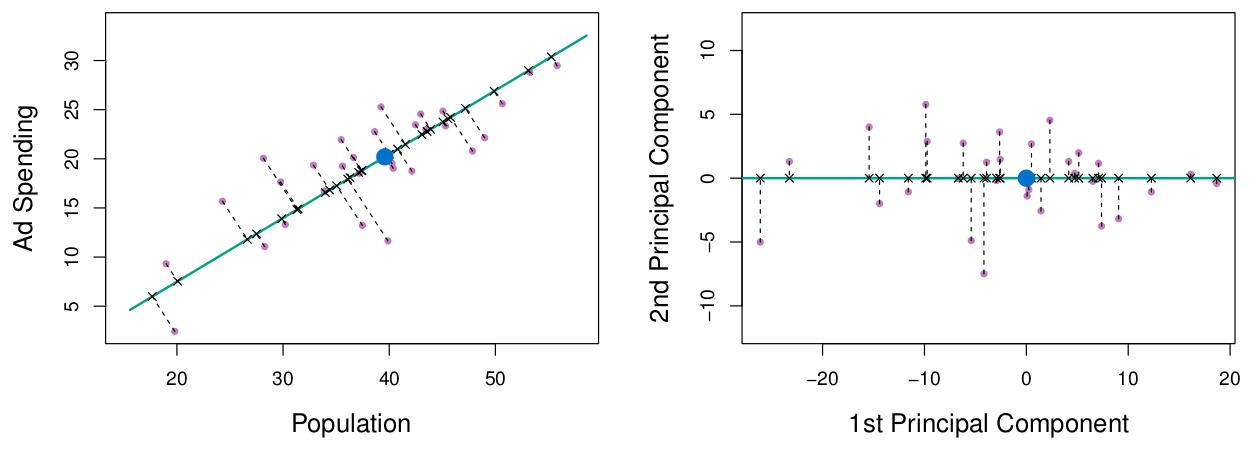
\includegraphics[width = .8\textwidth, align = c]{Fig6-15}
\begin{columns}
\column{.45\textwidth}
\centering
\InstructorList{
\item Think of this as rotated for now, 2nd PC on next slide
}
\column{.45\textwidth}
\centering
\InstructorList{
\item The score can be thought of as relation from the mean
\item $z_{i1}<0$ has below avg pop size as below avg ad spending
}

\end{columns}

\end{frame}
%--- Next Frame ---%
\begin{frame}[t]{The other principal components}
\centering
	% 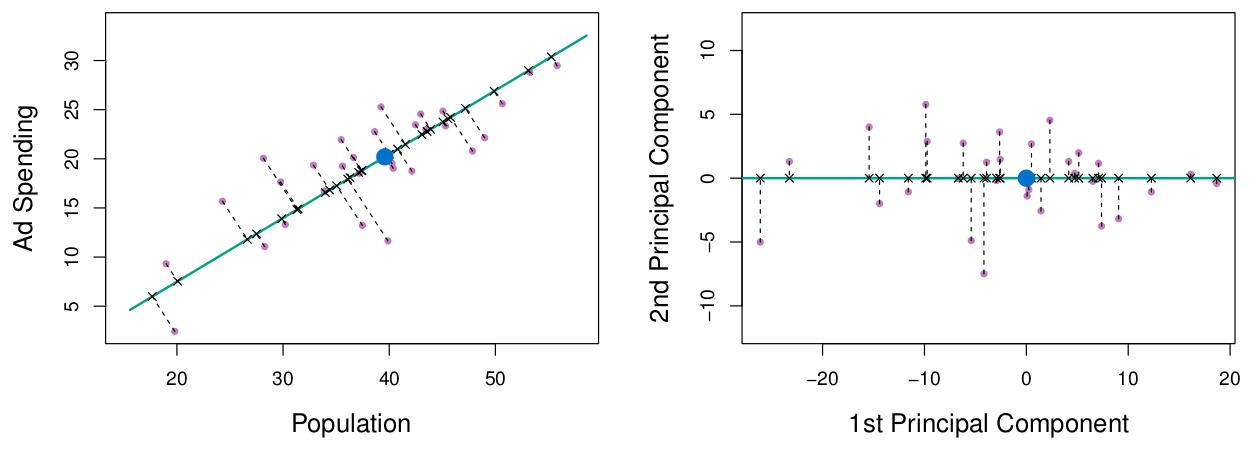
\includegraphics[width = .8\textwidth, align = c]{Fig6-15}
\begin{columns}
\column{.45\textwidth}
\centering
\InstructorList{
\item $Z_2$ is linear combo of variables uncorrelated to $Z_1$
\item Find the one that explains the most variance
\item Result: requires $Z_2$ to be orthogonal or perpendicular
\item[]
\item How does your compy do it? Fun with matrices, outside the scope of class, but you should be able to interpret the output
}


\column{.45\textwidth}
\centering
\InstructorNotes{
Draw the idea in 3D with circle of directions around a line in 3D
}
\end{columns}

\end{frame}
%--- Next Frame ---%
{
\setbeamercolor{background canvas}{bg=Apricot!25}
\begin{frame}[t]{Do PCA with Penguins}
\begin{columns}
\column{.45\textwidth}
\centering
\column{.45\textwidth}
\centering
\end{columns}
% LIZ START EDITING SLIDES HERE
\end{frame}
}
%--- Next Frame ---%






\begin{frame}[c]{TL;DR}

\begin{columns}
\column{.45\textwidth}
\centering
\textbf{PCA}
\begin{itemize}
	\item Unsupervised dimensionality reduction
	\item Choose component $Z_1$ in the direction of most variance using only $X_i$'s information
	\item Choose $Z_2$ and beyond by the same method after ``getting rid'' of info in the directions already explained
\end{itemize}
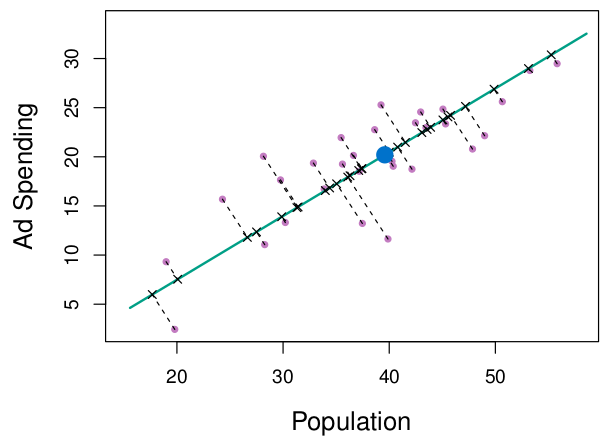
\includegraphics[width = .5\textwidth, align = c]{Fig6-15a}

\column{.45\textwidth}
\centering

% \textbf{PCR}
% \begin{itemize}
% 	\item Do PCA on input data 
% 	\item Do Linear Regression on chosen number of PCs. 
% 	\item Warning: Lose interpretability of the coefficients.
% \end{itemize}

% \begin{itemize}
% 	\item Supervised dimensionality reduction
% 	\item Choose component $Z_1$ by using simple regression coefficients of each $X_i$ onto $Y$
% 	\item Choose $Z_2$ and beyond by the same method after ``getting rid'' of info in the directions already explained
% 	\item Not a particular benefit, so usually default to PCA unless you have a good reason for this
% \end{itemize}
% 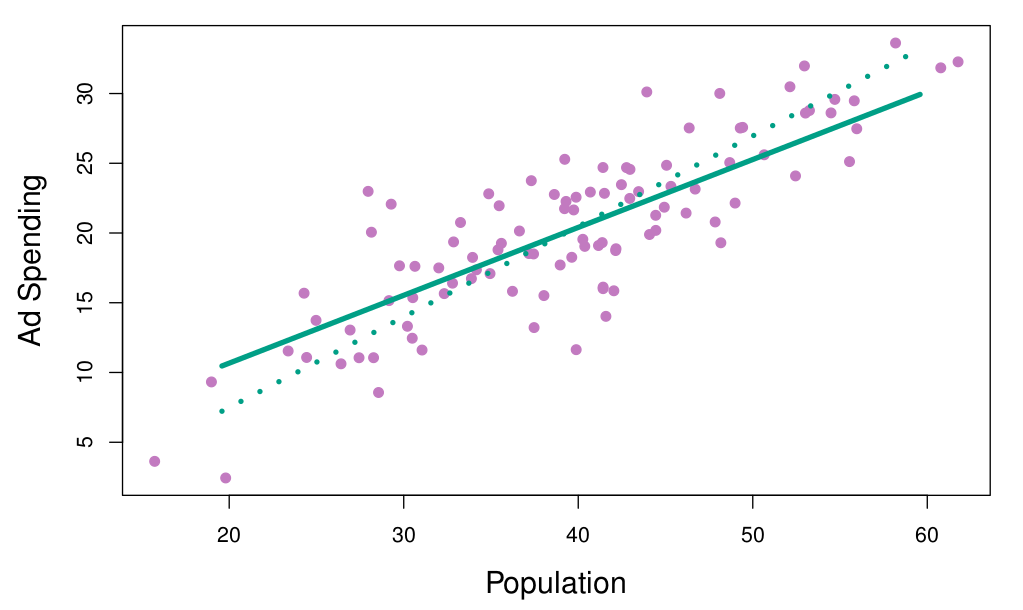
\includegraphics[width = .5\textwidth]{Fig6-21}
% 
\end{columns}

\end{frame}
%--- Next Frame ---%



\begin{frame}[t]{Next time}

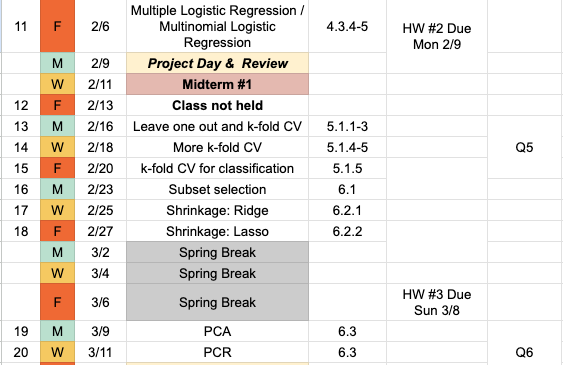
\includegraphics[align = c, width = .65\textwidth]{Schedule-S26-Lecs11_to_20}
	

% \begin{columns}
% \column{.45\textwidth}
% \centering

% \textbf{Next time:}

% \begin{itemize}
% 	\item
% Ch 6.4 Issues in High Dimensions
% \end{itemize}

% \column{.45\textwidth}
% \centering

% \textbf{This week:}
% \begin{itemize}

% 	\item Mon 3/14: 6.3 PCA and regression
% 	\item Weds 3/16: 6.4 High Dimensions
% 	\item Fri 3/18: 6.5 Lab
% 	\begin{itemize}
% 		\item Homework \#7 Due
% 		\item Covers Monday and Wednesday only
% 	\end{itemize}
% \end{itemize}
% 	\end{columns}

\end{frame}
%--- Next Frame ---%


\end{document}
